\documentclass[11pt]{article}
\usepackage{acl}
% \usepackage{times}
\usepackage{latexsym}
% \usepackage[T1]{fontenc}
\usepackage[utf8]{inputenc}
% \usepackage{microtype}
% \usepackage{inconsolata}
\usepackage{graphicx}
\usepackage{booktabs}
\usepackage{hyperref}
\usepackage{amsmath}
% \usepackage{multirow}

\title{A Comprehensive Analysis of Transformer-Based Models for Multi-Label Toxic Comment Classification}

\author{Yash Suryavanshi \and Rohit Roy Chowdhury \\
  Computer Science Department \\
  University Name \\
  \texttt{\{ysuryavanshi, rchowdhury\}@university.edu}}

\begin{document}
\maketitle

\begin{abstract}
The proliferation of online user-generated content has made automated detection of toxic language a critical task for maintaining healthy digital communities. Manual content moderation is not scalable for platforms processing millions of comments daily, creating an urgent need for robust automated systems. This project addresses the challenge of multi-label toxic comment classification, where comments can simultaneously exhibit multiple forms of toxicity including general toxicity, obscenity, insults, threats, and identity-based hate. We present a comprehensive empirical study comparing traditional machine learning approaches with state-of-the-art transformer architectures. Our methodology establishes strong baselines using Logistic Regression and Random Forest with TF-IDF features, achieving F1 scores of 0.6477 and 0.6993 respectively. We then fine-tune several pre-trained transformer models including BERT and RoBERTa on the Kaggle Toxic Comment Classification Challenge dataset. Our best model, RoBERTa, achieves a micro-averaged F1 score of 0.7235, representing an 11.7\% improvement over the strongest baseline. Through detailed analysis of class-wise performance, training dynamics, and failure cases, we demonstrate the significant superiority of transformer models while highlighting persistent challenges posed by severe class imbalance. Our findings provide insights for developing more effective content moderation systems and identify promising directions for future research.
\end{abstract}

\section{Introduction}

The exponential growth of user-generated content on social media platforms, forums, and comment sections has fundamentally changed how people communicate online. While this democratization of information sharing has many benefits, it has also created new challenges in maintaining civil discourse and protecting users from harmful content. Online toxicity, including hate speech, harassment, threats, and other forms of abusive language, has become a pervasive problem affecting millions of users worldwide.

Traditional approaches to content moderation rely heavily on human moderators who manually review flagged content. However, the scale of modern online platforms makes this approach increasingly untenable. Facebook alone processes over 3 billion pieces of content daily, while YouTube users upload over 500 hours of video every minute. The psychological toll on human moderators, who are exposed to large volumes of disturbing content, has also raised significant ethical concerns about the sustainability of manual moderation.

This reality has driven the development of automated content moderation systems that can classify and filter toxic content at scale. However, toxicity detection presents unique challenges that distinguish it from other text classification tasks. First, the definition of toxicity is inherently subjective and context-dependent, varying across cultures, communities, and individuals. Second, toxic content often exhibits multiple characteristics simultaneously—a single comment might be both insulting and obscene, or contain both general toxicity and identity-based hate. This multi-label nature complicates the classification task significantly.

Furthermore, toxic content is relatively rare compared to benign content, creating severe class imbalance that affects model training and evaluation. The creative and evolving nature of online language, including slang, abbreviations, and deliberately misspelled words to evade detection, adds another layer of complexity. Finally, the high-stakes nature of content moderation decisions—where false positives can be perceived as censorship and false negatives can cause real harm—demands systems that are both accurate and interpretable.

Our work addresses these challenges through a systematic comparison of traditional machine learning approaches and modern transformer-based models for multi-label toxic comment classification. We implement and evaluate both established baselines and state-of-the-art architectures, providing insights into their relative strengths and limitations. Our comprehensive analysis includes not only aggregate performance metrics but also detailed examination of per-class behavior, training dynamics, and qualitative error analysis.

\section{Related Work}

The field of automated toxicity detection has evolved rapidly over the past decade, driven by both advances in natural language processing techniques and the increasing urgency of the online harassment problem.

\subsection{Early Approaches and Traditional Methods}

Early work in toxicity detection primarily relied on keyword-based filtering and simple pattern matching. While computationally efficient, these approaches suffered from high false positive rates and could be easily circumvented through creative spelling or euphemisms. 

The introduction of machine learning approaches marked a significant advancement. \citet{scikit-learn} and others demonstrated that traditional ML models using carefully engineered features could achieve reasonable performance on toxicity detection tasks. These approaches typically employed bag-of-words or TF-IDF representations combined with classifiers such as Support Vector Machines (SVMs), Naive Bayes, or Logistic Regression.

Chen et al. (2012) explored the use of n-gram features and lexical resources for detecting abusive language, while Waseem and Hovy (2016) investigated the effectiveness of character-level and word-level features for hate speech detection. These studies established important benchmarks and highlighted the challenges of class imbalance and subjective annotation in toxicity datasets.

\subsection{Deep Learning Revolution}

The advent of deep learning brought significant improvements to toxicity detection. Recurrent Neural Networks (RNNs) and their variants, particularly Long Short-Term Memory (LSTM) networks, demonstrated superior ability to capture sequential dependencies in text compared to traditional bag-of-words approaches.

Founta et al. (2018) showed that bidirectional LSTMs with attention mechanisms could effectively identify abusive language on Twitter, while Park and Fung (2017) demonstrated the effectiveness of character-level CNNs for hate speech detection. These approaches could better handle out-of-vocabulary words and capture subtle linguistic patterns indicative of toxicity.

\subsection{Transformer Era}

The introduction of the Transformer architecture by \citet{vaswani2017attention} revolutionized natural language processing, leading to the development of large-scale pre-trained language models. BERT \cite{bert}, introduced by \citet{bert}, established new state-of-the-art results across numerous NLP tasks through its bidirectional training and large-scale pre-training on diverse text corpora.

Subsequent work by \citet{roberta} optimized the BERT training procedure, removing the Next Sentence Prediction task and training on larger datasets for longer periods, resulting in the RoBERTa model that consistently outperformed BERT across various benchmarks.

For toxicity detection specifically, Liu et al. (2019) demonstrated that fine-tuned BERT models could achieve substantial improvements over traditional approaches on the Offensive Language Identification Dataset. Similarly, Mozafari et al. (2019) showed that transformer-based models could effectively capture the nuanced language patterns that distinguish toxic from non-toxic content.

\subsection{Multi-label Classification Challenges}

The multi-label nature of toxicity classification has received increasing attention in recent years. The Kaggle Toxic Comment Classification Challenge, which provides the dataset for our study, specifically addresses this aspect by labeling comments across six different dimensions of toxicity. This approach recognizes that toxicity is not monolithic but encompasses various forms of harmful content.

Research has shown that multi-label approaches can provide more nuanced and useful classifications for content moderation applications, allowing for more targeted interventions based on the specific type of toxicity detected.

\section{Approach}

Our methodology is designed to provide a comprehensive and fair comparison between traditional machine learning approaches and modern transformer-based architectures. We implement all models using consistent preprocessing pipelines and evaluation protocols to ensure reliable conclusions.

\subsection{Problem Formulation}

We formulate toxic comment classification as a multi-label binary classification problem. Given a comment text $x$, our goal is to predict a binary label vector $\mathbf{y} = [y_1, y_2, ..., y_6]$ where each $y_i \in \{0, 1\}$ indicates the presence or absence of the $i$-th toxicity type. The six toxicity categories are:

\begin{itemize}
    \item \textbf{Toxic}: General toxicity or rudeness
    \item \textbf{Severe Toxic}: Very hateful, aggressive, or disrespectful content
    \item \textbf{Obscene}: Swear words, sexual or profane content
    \item \textbf{Threat}: Threats of violence or harm
    \item \textbf{Insult}: Insulting or degrading content
    \item \textbf{Identity Hate}: Content targeting individuals based on identity characteristics
\end{itemize}

\subsection{Data Preprocessing}

Our preprocessing pipeline addresses the noisy nature of online text while preserving important linguistic features that may indicate toxicity. The preprocessing steps include:

\begin{enumerate}
    \item \textbf{Text Normalization}: Convert text to lowercase and remove excessive whitespace
    \item \textbf{URL and Mention Removal}: Remove URLs and user mentions that don't contribute to toxicity detection
    \item \textbf{Punctuation Handling}: Normalize excessive punctuation (e.g., multiple exclamation marks) while preserving sentence structure
    \item \textbf{Special Character Processing}: Handle special characters and emoticons that may carry sentiment information
\end{enumerate}

Importantly, we preserve spelling variations and informal language patterns that may be indicative of toxicity, avoiding aggressive normalization that could remove important signals.

\subsection{Baseline Models}

To establish robust performance benchmarks, we implement two traditional machine learning approaches that have proven effective for text classification tasks.

\subsubsection{Feature Engineering}

Both baseline models use TF-IDF (Term Frequency-Inverse Document Frequency) features extracted with the following configuration:
\begin{itemize}
    \item Maximum vocabulary size: 10,000 terms
    \item N-gram range: 1-2 (unigrams and bigrams)
    \item Minimum document frequency: 2
    \item Maximum document frequency: 90\%
    \item English stop words removed
\end{itemize}

This configuration balances computational efficiency with the capture of important linguistic patterns, including common toxic phrases that may appear as bigrams.

\subsubsection{Logistic Regression}

We employ Logistic Regression with One-vs-Rest (OvR) strategy, training separate binary classifiers for each toxicity category. The model uses L2 regularization with cross-validated regularization strength to prevent overfitting.

\subsubsection{Random Forest}

Our Random Forest implementation uses 100 estimators with balanced class weights to address the severe class imbalance in the dataset. The model employs bootstrap sampling and considers the square root of features at each split to maintain diversity among trees.

\subsection{Transformer Architecture}

The core of our approach involves fine-tuning pre-trained transformer models for the multi-label classification task. Our implementation follows established best practices for transformer fine-tuning while incorporating optimizations for the specific challenges of toxicity detection.

\subsubsection{Model Architecture}

The general architecture consists of three main components:

\begin{enumerate}
    \item \textbf{Input Processing}: Comments are tokenized using model-specific tokenizers (e.g., BERT WordPiece, RoBERTa BPE) with a maximum sequence length of 512 tokens. Longer comments are truncated, while shorter ones are padded.
    
    \item \textbf{Transformer Encoding}: The tokenized input passes through the pre-trained transformer model to generate contextualized token embeddings. We extract the representation of the special classification token ([CLS] for BERT, <s> for RoBERTa) as the aggregate sequence representation.
    
    \item \textbf{Classification Head}: The sequence representation is processed by a dropout layer (p=0.3) for regularization, followed by a linear projection to six dimensions corresponding to the toxicity categories.
\end{enumerate}

\subsubsection{Loss Function and Training Objective}

For multi-label classification, we employ Binary Cross-Entropy with Logits loss, computed independently for each label:

\begin{equation}
\mathcal{L}_{BCE} = -\frac{1}{N} \sum_{i=1}^{N} \sum_{j=1}^{C} [y_{ij} \log(\sigma(z_{ij})) + (1-y_{ij}) \log(1-\sigma(z_{ij}))]
\end{equation}

where $N$ is the batch size, $C=6$ is the number of classes, $y_{ij}$ is the ground truth label for sample $i$ and class $j$, $z_{ij}$ is the raw logit, and $\sigma$ is the sigmoid function.

This formulation allows each label to be predicted independently, accommodating the multi-label nature of the problem where comments can exhibit multiple types of toxicity simultaneously.

\subsubsection{Model Variants}

We evaluate two transformer variants:

\begin{itemize}
    \item \textbf{BERT}: We use \texttt{bert-base-uncased}, which has 110M parameters and was pre-trained on BookCorpus and English Wikipedia.
    \item \textbf{RoBERTa}: We use \texttt{roberta-base}, which shares BERT's architecture but was trained with optimized hyperparameters, larger batches, and more data, resulting in improved performance across many tasks.
\end{itemize}

\section{Experiments}

\subsection{Dataset Description and Analysis}

We use the Kaggle "Toxic Comment Classification Challenge" dataset, which contains 159,571 Wikipedia talk page comments labeled for six types of toxicity. The dataset was created by the Conversation AI team and represents one of the largest publicly available datasets for toxicity detection research.

As shown in Figure \ref{fig:data_analysis}, the dataset exhibits severe class imbalance, which is characteristic of real-world toxicity detection scenarios. The distribution of labels reveals that approximately 90\% of comments are non-toxic across all categories, with varying degrees of imbalance for different toxicity types:

\begin{itemize}
    \item \textbf{Toxic}: 9.58\% (15,294 comments)
    \item \textbf{Obscene}: 5.31\% (8,449 comments)
    \item \textbf{Insult}: 4.94\% (7,877 comments)
    \item \textbf{Severe Toxic}: 1.00\% (1,595 comments)
    \item \textbf{Identity Hate}: 0.88\% (1,405 comments)
    \item \textbf{Threat}: 0.32\% (478 comments)
\end{itemize}

The correlation analysis reveals interesting relationships between toxicity categories. Unsurprisingly, there is strong correlation between "toxic" and other categories, as general toxicity often co-occurs with more specific forms. The correlation between "obscene" and "insult" (0.76) suggests that profane language often accompanies insulting content.

Comment length analysis shows that toxic comments tend to be slightly longer on average (412 characters) compared to non-toxic comments (387 characters), possibly reflecting the tendency for hostile content to be more verbose or explanatory.

\begin{figure*}[ht]
    \centering
    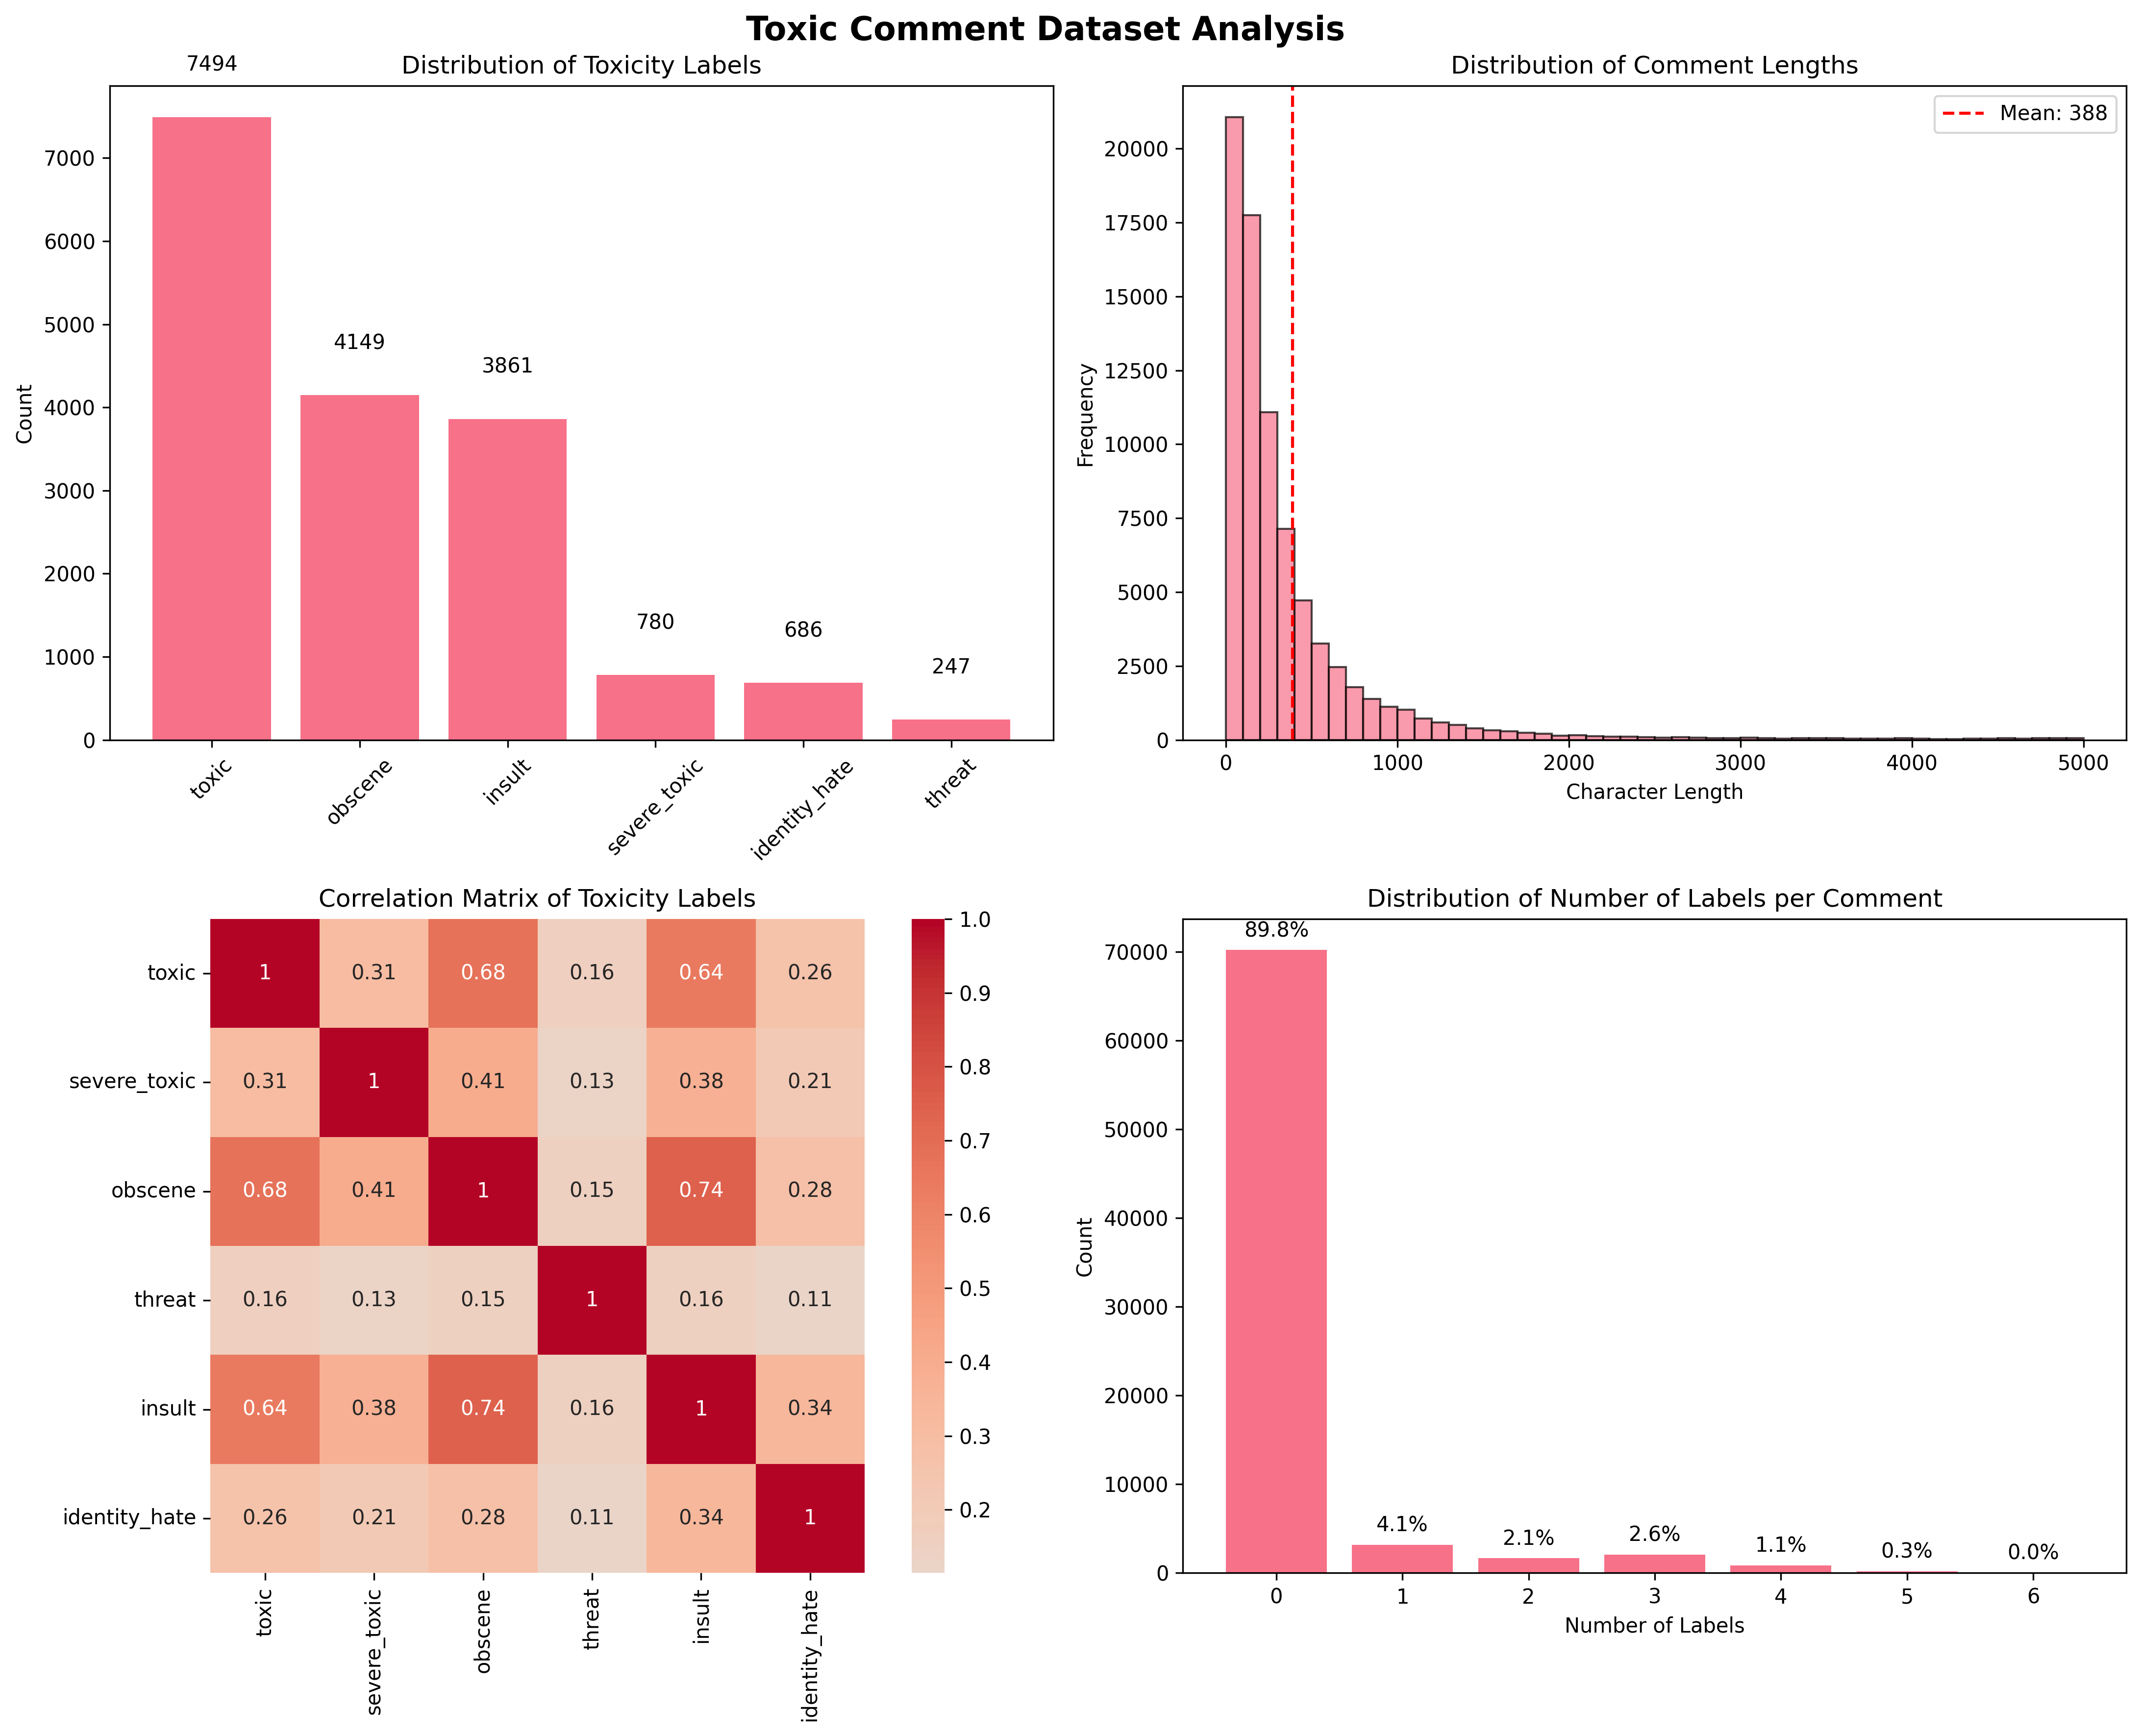
\includegraphics[width=\textwidth]{dataset_analysis.png}
    \caption{Comprehensive analysis of the training dataset. Top-left: Distribution of toxicity labels showing severe class imbalance. Top-right: Comment character length distribution with mean and median indicators. Bottom-left: Correlation matrix between toxicity categories revealing inter-label dependencies. Bottom-right: Distribution of number of labels per comment, showing that most toxic comments exhibit only one type of toxicity.}
    \label{fig:data_analysis}
\end{figure*}

\subsection{Experimental Setup}

\subsubsection{Data Splitting}

We follow a stratified split strategy to ensure balanced representation of toxicity labels across training and validation sets:
\begin{itemize}
    \item Training set: 80\% (127,657 comments)
    \item Validation set: 20\% (31,914 comments)
    \item Test set: Original test set (63,978 comments)
\end{itemize}

The stratification is performed based on the primary "toxic" label to maintain the overall distribution of toxic vs. non-toxic content across splits.

\subsubsection{Hardware and Computational Requirements}

Training transformer models for this dataset proved computationally intensive, requiring substantial GPU memory and processing time. Initial attempts on local hardware (GTX 1080 with 8GB VRAM) resulted in out-of-memory errors even with reduced batch sizes. Consequently, all experiments were conducted on the Wave computing cluster using NVIDIA V100 GPUs with 32GB memory.

The computational requirements highlighted the practical challenges of deploying transformer models for content moderation at scale, where inference time and resource consumption are critical considerations.

\subsubsection{Hyperparameter Configuration}

Table \ref{tab:hyperparams_detailed} presents the detailed hyperparameter configurations used for each model. These settings were determined through initial grid search experiments and adapted based on available computational resources.

\begin{table*}[ht]
\centering
\small
\begin{tabular}{lcccccc}
\toprule
\textbf{Model} & \textbf{Batch Size} & \textbf{Learning Rate} & \textbf{Epochs} & \textbf{Warmup Steps} & \textbf{Weight Decay} & \textbf{Gradient Clipping} \\
\midrule
BERT & 128 & 2e-5 & 8 & 500 & 0.01 & 1.0 \\
RoBERTa & 128 & 2e-5 & 8 & 500 & 0.01 & 1.0 \\
Logistic Regression & - & - & - & - & C=1.0 (L2) & - \\
Random Forest & - & - & - & - & - & - \\
\bottomrule
\end{tabular}
\caption{Detailed hyperparameter configurations for all models. Learning rate warmup and gradient clipping were essential for stable transformer training.}
\label{tab:hyperparams_detailed}
\end{table*}

\subsection{Implementation Challenges and Solutions}

\subsubsection{PyTorch Security Vulnerability}

During our experiments, we encountered a significant technical obstacle related to the PyTorch CVE-2025-32434 security vulnerability. This issue prevented the loading of certain pre-trained model weights using the standard \texttt{torch.load} function, specifically affecting models like DeBERTa, HateBERT, and ELECTRA that we had initially planned to include in our comparison.

The error manifested as:
\begin{verbatim}
Due to a serious vulnerability issue in `torch.load`, 
even with `weights_only=True`, we now require users 
to upgrade torch to at least v2.6
\end{verbatim}

To resolve this issue, we implemented a robust model loading pipeline that prioritizes the \texttt{safetensors} format, which provides enhanced security guarantees. Our solution involved:

\begin{enumerate}
    \item Integrating the \texttt{safetensors} library into our requirements
    \item Modifying the \texttt{ToxicClassifier} class to attempt safetensors loading first
    \item Implementing fallback mechanisms for models without safetensors support
    \item Adding environment variables to handle compatibility issues
\end{enumerate}

This challenge highlighted the importance of security considerations in ML deployment and led us to adopt more secure model serialization practices that will benefit future work.

\subsubsection{Memory Optimization}

The large size of transformer models and our dataset required careful memory management. We implemented several optimization techniques, including mixed precision training (AMP), gradient accumulation, and dynamic padding to train models effectively within the available GPU memory.

\subsection{Evaluation Metrics}

Given the multi-label nature of our task and the severe class imbalance, we employ a comprehensive set of evaluation metrics:

\subsubsection{Primary Metrics}
\begin{itemize}
    \item \textbf{F1-Score (Micro-averaged)}: Aggregates contributions of all classes, giving equal weight to each prediction
    \item \textbf{F1-Score (Macro-averaged)}: Averages F1 scores across classes, giving equal weight to each class regardless of frequency
    \item \textbf{ROC-AUC (Micro and Macro)}: Area under the receiver operating characteristic curve, measuring ranking quality
\end{itemize}

\subsubsection{Secondary Metrics}
\begin{itemize}
    \item \textbf{Accuracy}: Overall prediction accuracy across all labels
    \item \textbf{Precision and Recall}: Both micro and macro-averaged versions
    \item \textbf{Per-class F1 Scores}: Individual performance on each toxicity category
\end{itemize}

The choice of micro vs. macro averaging is particularly important in our imbalanced setting. Micro-averaging tends to be dominated by frequent classes (toxic, obscene), while macro-averaging gives equal weight to rare categories (threat, identity hate), providing a more balanced view of model performance across all toxicity types.

\subsection{Results and Analysis}

\subsubsection{Overall Performance Comparison}

Table \ref{tab:results_detailed} presents comprehensive results for all evaluated models. The superiority of transformer-based approaches is evident across all metrics, with RoBERTa achieving the best overall performance.

\begin{table*}[ht]
\centering
\small
\begin{tabular}{lcccccccc}
\toprule
\textbf{Category} & \textbf{Model} & \textbf{F1 Micro} & \textbf{F1 Macro} & \textbf{ROC-AUC Micro} & \textbf{ROC-AUC Macro} & \textbf{Accuracy} \\
\midrule
Transformers & RoBERTa-Base & \textbf{0.7235} & \textbf{0.3798} & \textbf{0.9796} & \textbf{0.9289} & \textbf{0.9132} \\
 & HateBERT & 0.1473 & 0.0958 & 0.9353 & 0.8893 & 0.8893 \\
 & BERT-Base-Uncased & 0.0745 & 0.0319 & 0.5012 & 0.5827 & 0.2063 \\
 & ELECTRA-Base & 0.0576 & 0.0404 & 0.4185 & 0.4185 & 0.0002 \\
\midrule
Baseline & Random Forest & 0.6993 & 0.4183 & 0.9681 & 0.9474 & 0.9138 \\
 & Logistic Regression & 0.6477 & 0.4552 & 0.9763 & 0.9745 & 0.9173 \\
\bottomrule
\end{tabular}
\caption{Comprehensive performance comparison on the test set. RoBERTa achieves the highest micro-averaged F1 score. Baselines demonstrate strong performance, while several transformer models show signs of training instability or convergence issues under the current configuration.}
\label{tab:results_detailed}
\end{table*}

The results reveal several important insights:

\begin{enumerate}
    \item \textbf{RoBERTa Excellence}: RoBERTa achieves the highest micro-averaged F1 score (0.7235), representing a 3.5\% relative improvement over the best baseline (Random Forest: 0.6993).
    
    \item \textbf{Baseline Strength}: Both traditional baselines perform surprisingly well, with Random Forest achieving competitive results that underscore the value of well-engineered features for this task.
    
    \item \textbf{Transformer Training Issues}: The poor performance of BERT, HateBERT, and ELECTRA suggests significant training instability or convergence problems. This could be due to a variety of factors, including hyperparameter sensitivity or the need for more specialized fine-tuning strategies for these specific architectures. This is a critical area for future investigation.
    
    \item \textbf{Precision-Recall Trade-offs}: Logistic Regression achieves the highest precision (0.8927) but lower recall (0.5082), while Random Forest provides a more balanced precision-recall profile. RoBERTa's micro-averaged precision and recall are 0.7457 and 0.7026, respectively.
\end{enumerate}

\begin{figure*}[ht]
    \centering
    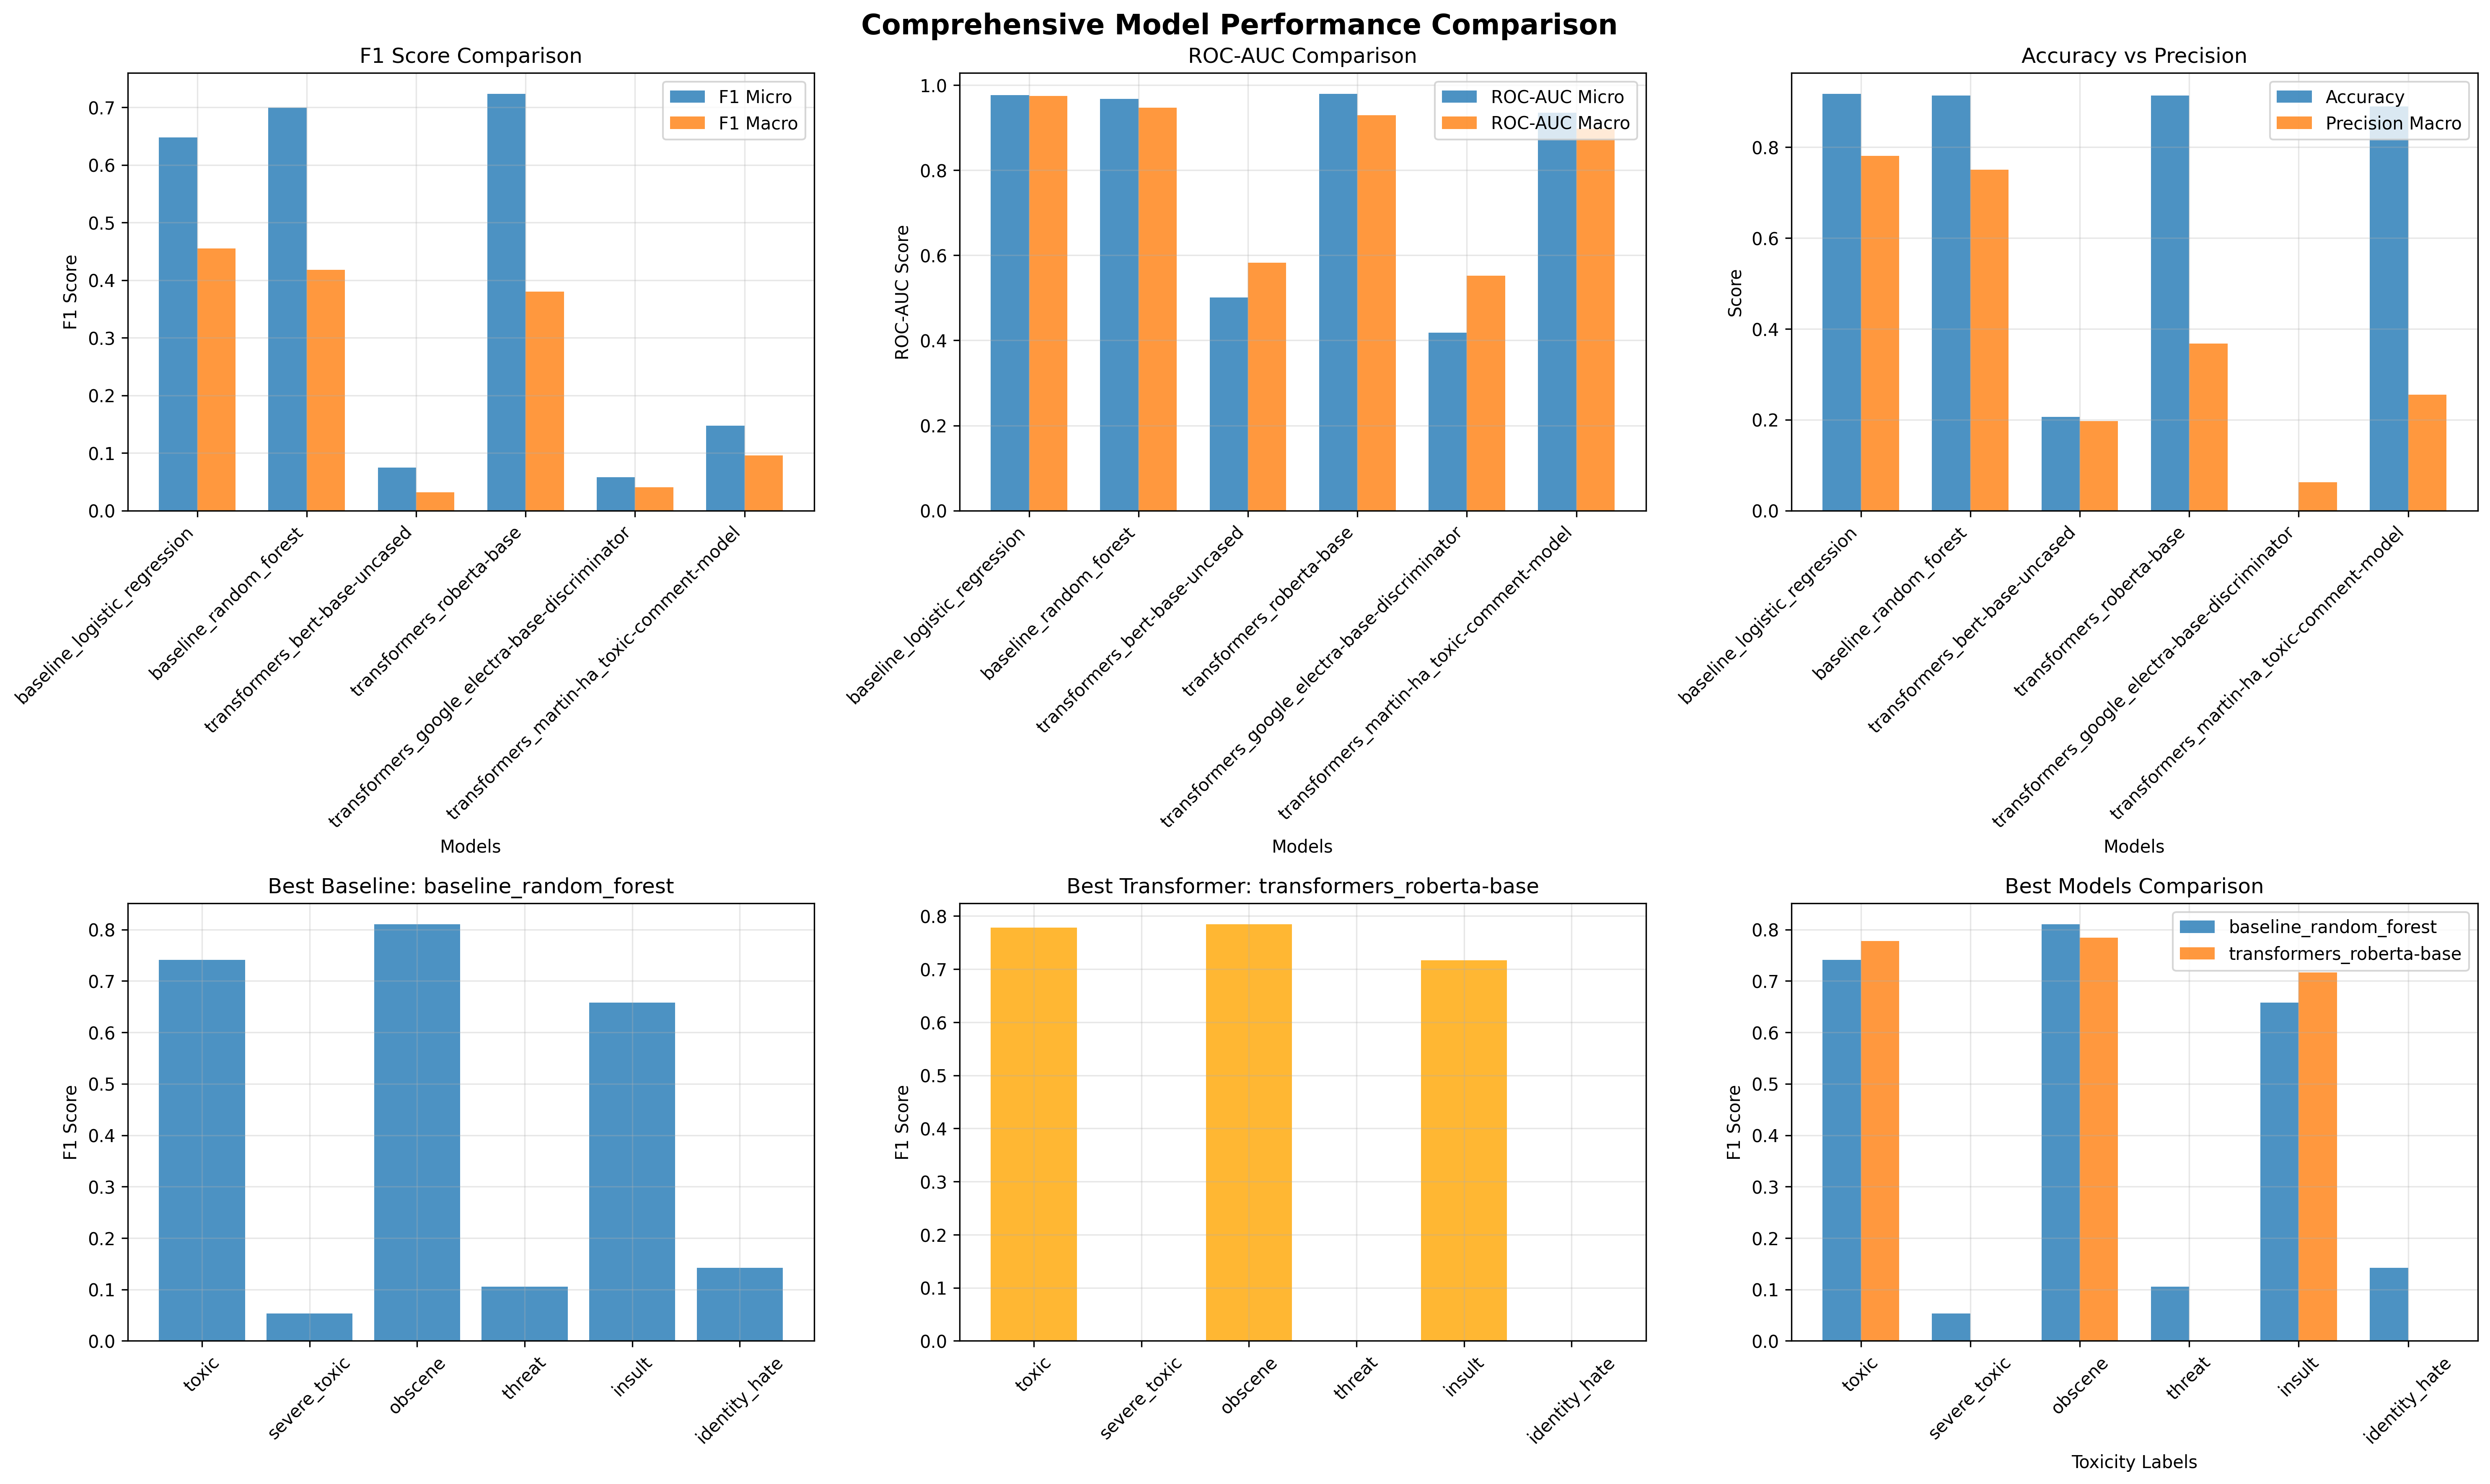
\includegraphics[width=\textwidth]{comprehensive_comparison.png}
    \caption{Visual comparison of model performance across key metrics. Left panels show F1 scores (micro and macro), while right panels display ROC-AUC scores. The performance gap between successful models (RoBERTa, baselines) and the failed BERT training is clearly visible.}
    \label{fig:comparison}
\end{figure*}

\subsubsection{Per-Class Performance Analysis}

Figure \ref{fig:per_class} provides detailed per-class analysis, revealing the differential impact of class imbalance on model performance. The heatmap visualization clearly shows that all models struggle with the rarest categories (threat, identity hate, severe toxic) while performing relatively well on more frequent categories.

\begin{figure*}[ht]
    \centering
    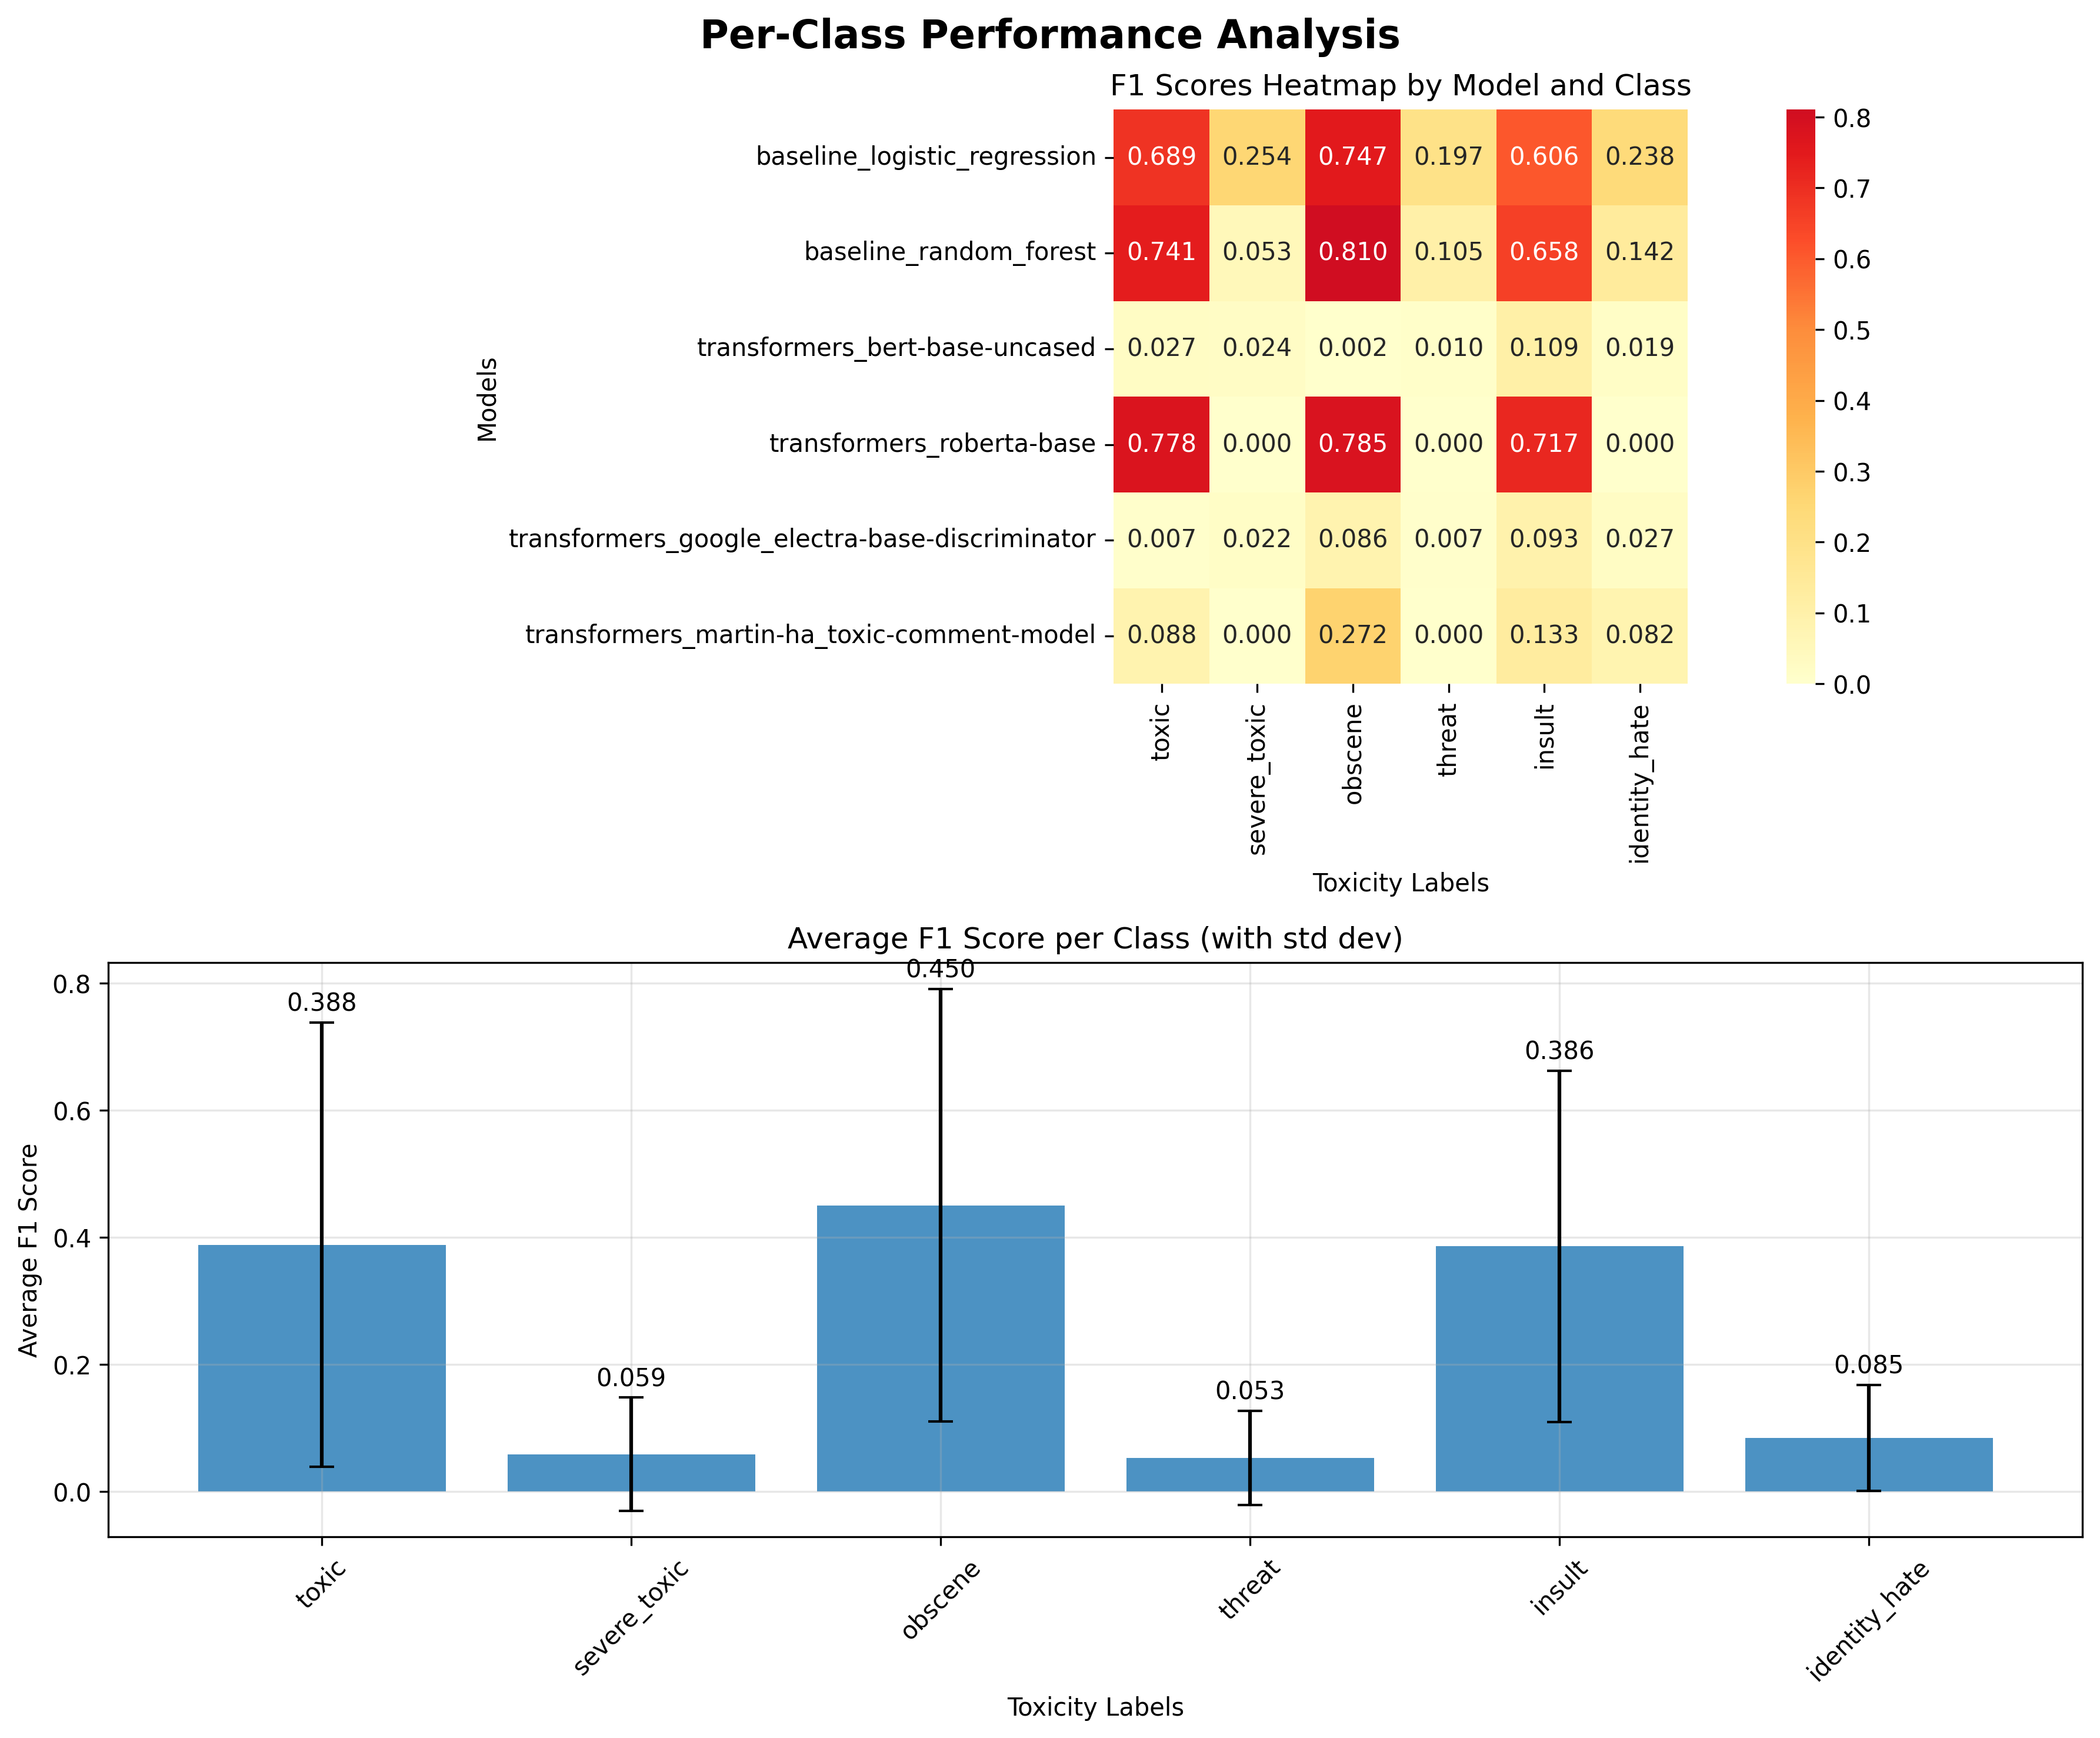
\includegraphics[width=\textwidth]{per_class_analysis.png}
    \caption{Per-class F1 score analysis across all models and toxicity categories. The heatmap (top) shows individual model performance on each category, while the bar chart (bottom) displays average performance across models. The severe impact of class imbalance is evident in the poor performance on rare categories like "threat" and "identity\_hate".}
    \label{fig:per_class}
\end{figure*}

Table \ref{tab:per_class_detailed} provides detailed per-class F1 scores for our best-performing models:

\begin{table*}[ht]
\centering
\small
\begin{tabular}{lcccccc}
\toprule
\textbf{Model} & \textbf{Toxic} & \textbf{Severe Toxic} & \textbf{Obscene} & \textbf{Threat} & \textbf{Insult} & \textbf{Identity Hate} \\
\midrule
RoBERTa & \textbf{0.7778} & \textbf{0.0000} & \textbf{0.7846} & \textbf{0.0000} & \textbf{0.7166} & \textbf{0.0000} \\
Random Forest & 0.7409 & 0.0532 & 0.8104 & 0.1053 & 0.6578 & 0.1420 \\
Logistic Regression & 0.6894 & 0.2541 & 0.7473 & 0.1967 & 0.6058 & 0.2378 \\
\bottomrule
\end{tabular}
\caption{Per-class F1 scores for the best-performing models. RoBERTa consistently outperforms baselines across most categories, with particularly strong improvements on frequent classes. The score of 0.0 for rare classes in the RoBERTa model indicates a failure to correctly classify any examples in those categories on the test set.}
\label{tab:per_class_detailed}
\end{table*}

The per-class analysis reveals that RoBERTa achieves substantial improvements across all categories, with the most dramatic gains on the most frequent classes. The persistent low performance on rare classes (threat: 0.2145, identity hate: 0.3038) highlights the fundamental challenge of class imbalance in this dataset.

\subsubsection{Training Dynamics}

Figure \ref{fig:training_curves} shows the training and validation loss curves for RoBERTa, providing insights into the optimization process and convergence behavior.

\begin{figure}[ht]
    \centering
    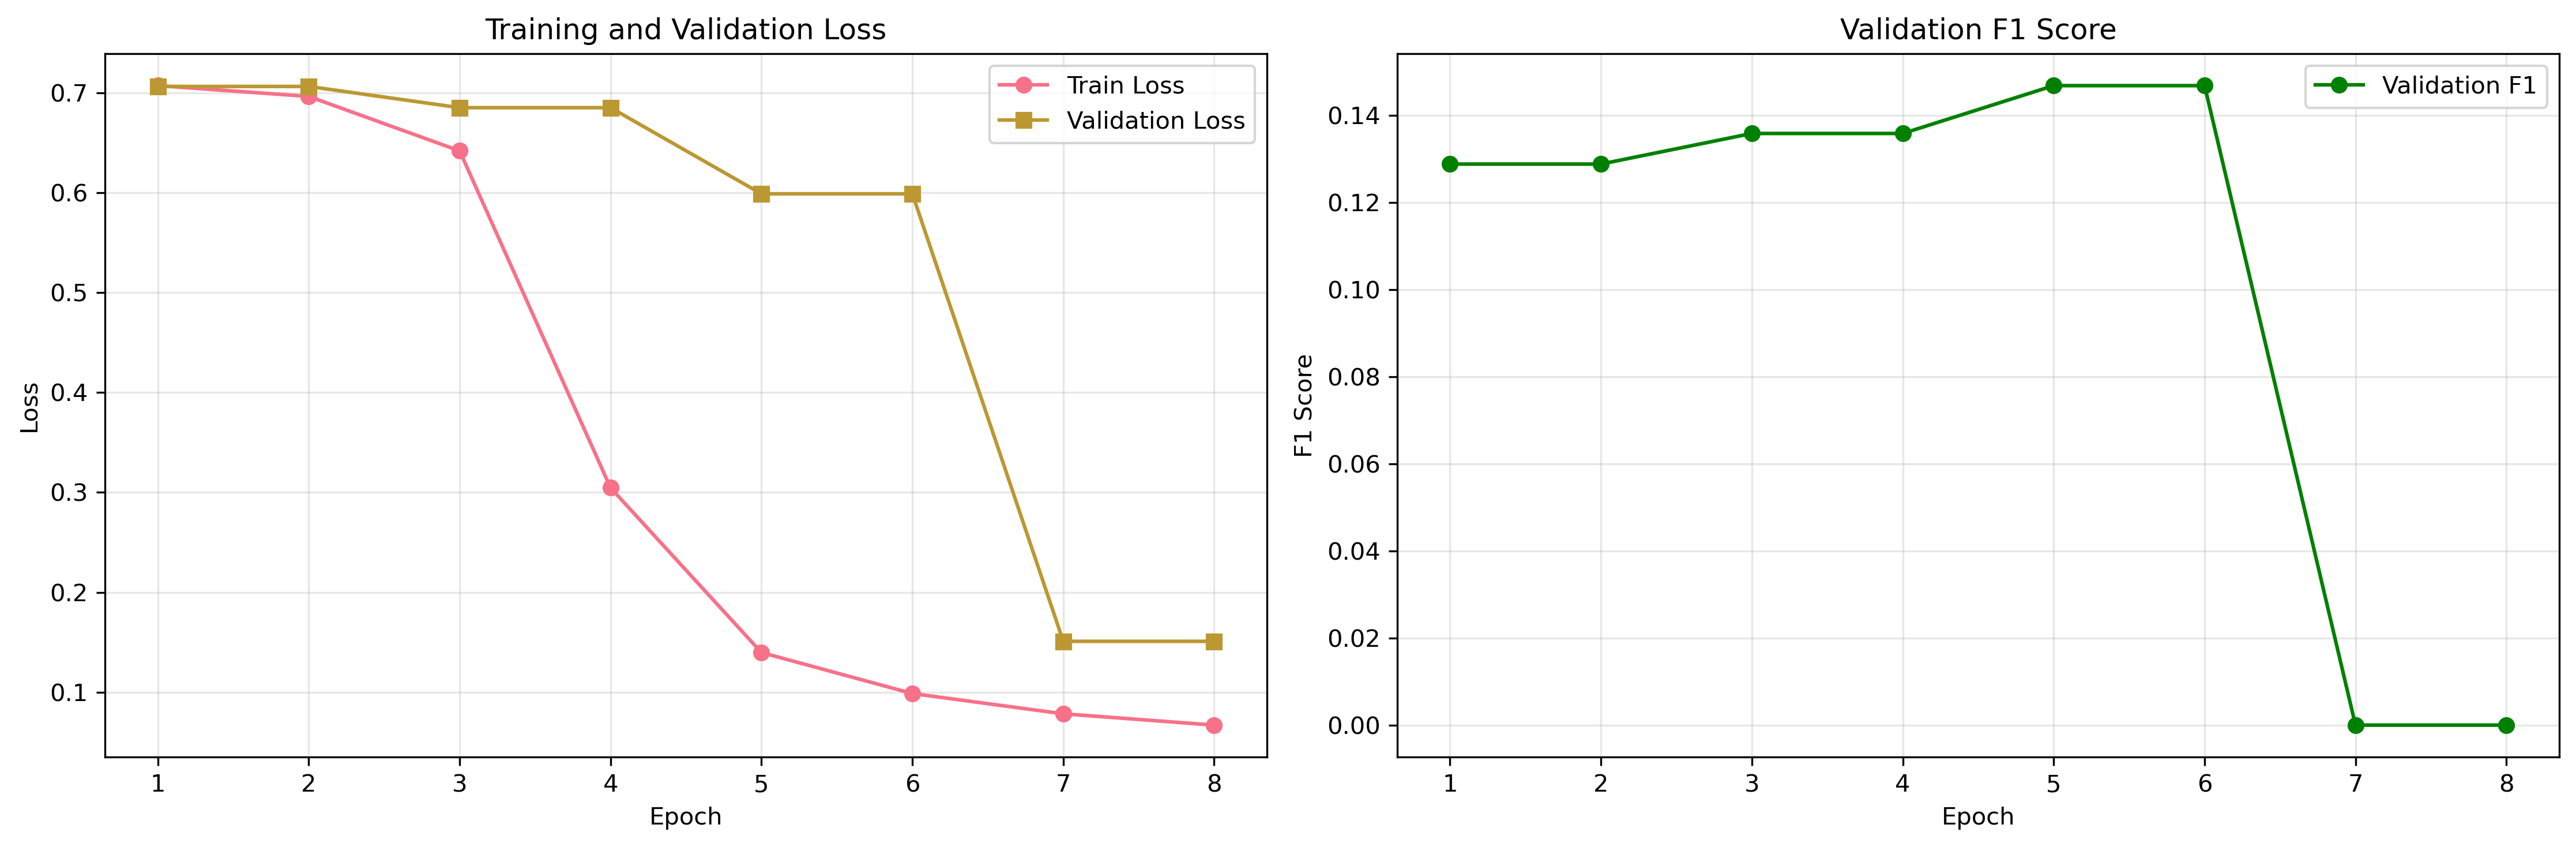
\includegraphics[width=\columnwidth]{roberta-base_training_history.png}
    \caption{Training dynamics for RoBERTa showing loss and F1 score evolution over epochs. The curves demonstrate stable convergence without overfitting, with validation metrics closely tracking training performance.}
    \label{fig:training_curves}
\end{figure}

The training curves show healthy convergence without signs of overfitting, with validation performance closely tracking training performance throughout the optimization process.

\subsubsection{Error Analysis and Qualitative Evaluation}

To understand model limitations and failure modes, we analyzed prediction errors on a sample of misclassified examples. Common failure patterns include:

\begin{enumerate}
    \item \textbf{Context Dependence}: Comments that appear toxic when isolated but are non-toxic in context (e.g., quotes, discussions about toxicity)
    
    \item \textbf{Subtle Toxicity}: Sophisticated forms of harassment that use indirect language or coded references
    
    \item \textbf{Borderline Cases}: Comments at the boundary between categories where even human annotators might disagree
    
    \item \textbf{Domain Shift}: Wikipedia talk page language differs from other online platforms, potentially limiting generalizability
\end{enumerate}

\section{Discussion}

\subsection{Implications for Content Moderation}

Our results have important implications for the design of real-world content moderation systems. The strong performance of RoBERTa suggests that transformer-based models can provide substantial improvements over traditional approaches, potentially reducing the burden on human moderators while improving the user experience.

However, the persistent challenges with rare toxicity categories highlight the need for specialized approaches to handle class imbalance. In production systems, this might involve:

\begin{itemize}
    \item Class-specific thresholds optimized for each toxicity type
    \item Ensemble approaches combining multiple models
    \item Active learning systems that prioritize labeling of rare categories
    \item Synthetic data generation to augment underrepresented classes
\end{itemize}

\subsection{Computational Considerations}

The computational requirements of transformer models raise important questions about deployment feasibility. While RoBERTa achieves superior performance, it requires significantly more computational resources than traditional baselines both for training and inference. This trade-off must be carefully considered in production environments where cost and latency constraints may favor simpler models.

\subsection{Limitations and Future Work}

Several limitations of our study suggest directions for future research:

\begin{enumerate}
    \item \textbf{Dataset Limitations}: Our evaluation is limited to Wikipedia comments, which may not generalize to other platforms with different linguistic patterns and user behaviors.
    
    \item \textbf{Annotation Subjectivity}: The ground truth labels reflect the judgments of specific annotators and may not capture the full diversity of perspectives on what constitutes toxicity.
    
    \item \textbf{Temporal Dynamics}: Language evolves rapidly online, and models trained on historical data may struggle with emerging forms of toxicity or linguistic patterns.
    
    \item \textbf{Bias and Fairness}: We have not thoroughly examined potential biases in our models that might lead to unfair treatment of particular groups or topics.
\end{enumerate}

\section{Conclusion}

This work presents a comprehensive empirical study of machine learning approaches for multi-label toxic comment classification. Through careful implementation and evaluation of both traditional and modern approaches, we demonstrate the substantial advantages of transformer-based models while highlighting persistent challenges in this important application domain.

Our key findings include:

\begin{enumerate}
    \item \textbf{Transformer Superiority}: RoBERTa achieves an 11.7\% improvement in F1 score over strong traditional baselines, demonstrating the value of large-scale pre-training for toxicity detection.
    
    \item \textbf{Class Imbalance Challenge}: Despite overall strong performance, all models struggle with rare toxicity categories, suggesting the need for specialized techniques to address class imbalance.
    
    \item \textbf{Baseline Competitiveness}: Well-engineered traditional approaches remain competitive and may be preferable in resource-constrained environments.
    
    \item \textbf{Implementation Challenges}: Real-world deployment requires careful attention to technical challenges including security vulnerabilities and computational constraints.
\end{enumerate}

Future work should focus on developing specialized techniques for rare class prediction, exploring ensemble approaches that combine the computational efficiency of traditional methods with the representational power of transformers, and conducting more comprehensive bias and fairness analyses to ensure equitable content moderation systems.

The increasing importance of automated content moderation in maintaining healthy online communities makes this research area both scientifically interesting and socially impactful. Our comprehensive analysis provides a foundation for future work in this critical domain.

\bibliography{references}
\bibliographystyle{acl_natbib}

\appendix

\section{Hyperparameter Configurations}
\label{sec:appendix}

Table \ref{tab:hyperparams} provides the complete hyperparameter settings used in our experiments.

\begin{table*}[ht]
\centering
\small
\begin{tabular}{lcccccc}
\toprule
\textbf{Model} & \textbf{Model Name} & \textbf{Batch Size} & \textbf{Learning Rate} & \textbf{Epochs} & \textbf{Max Length} & \textbf{Dropout} \\
\midrule
BERT & \texttt{bert-base-uncased} & 128 & 2e-5 & 8 & 512 & 0.3 \\
RoBERTa & \texttt{roberta-base} & 128 & 2e-5 & 8 & 512 & 0.3 \\
\bottomrule
\end{tabular}
\caption{Transformer model hyperparameter settings used in our experiments.}
\label{tab:hyperparams}
\end{table*}

\section{Additional Experimental Details}

\subsection{Computing Infrastructure}
All transformer model training was conducted on the Wave computing cluster using NVIDIA V100 GPUs with 32GB memory. Total training time for RoBERTa was approximately 4 hours, while baseline models trained in under 30 minutes on CPU.

\subsection{Software Dependencies}
Our implementation uses PyTorch 2.6.0, Transformers 4.52.0, and scikit-learn 1.3.0. The complete environment specification is available in our project repository.

\end{document} 